\section{Plasma}
El plasma es uno de los cuatro estados fundamentales de la materia, junto con sólido, líquido y gas. A diferencia de estos estados, el plasma se caracteriza por la presencia de partículas cargadas eléctricamente, como iones y electrones, que se comportan de manera colectiva \cite{plasma1}.
\subsection{Propiedades del plasma}
    \subsubsection{Carga electrica}
    La carga eléctrica en el plasma es un fenómeno fundamental que surge de la ionización de los átomos y moléculas presentes en el gas. Cuando se aplica suficiente energía al gas, algunos electrones son arrancados de sus órbitas alrededor de los núcleos atómicos, generando iones positivos (átomos con pérdida de electrones) y electrones libres. Esta separación de cargas crea un ambiente altamente conductor eléctricamente, similar a un gas de electrones y iones. La existencia de estas cargas libres permite que el plasma responda a campos eléctricos y magnéticos, y es la base de muchas de sus aplicaciones prácticas.
    \subsubsection{Temperatura}
    La temperatura elevada en el plasma es una consecuencia directa de la alta energía cinética de las partículas cargadas presentes. En términos simples, la temperatura es una medida de la energía promedio de movimiento de las partículas en un sistema. En un plasma, las partículas cargadas, como electrones e iones, tienen velocidades extremadamente altas debido a la gran cantidad de energía proporcionada durante la ionización. La temperatura del plasma puede variar significativamente según la aplicación y el entorno en el que se encuentre. Por ejemplo, en experimentos de fusión nuclear, se buscan temperaturas del orden de millones de grados Celsius para replicar las condiciones del núcleo solar.
    \subsubsection{Reactividad}
    La temperatura elevada en el plasma es una consecuencia directa de la alta energía cinética de las partículas cargadas presentes. En términos simples, la temperatura es una medida de la energía promedio de movimiento de las partículas en un sistema. En un plasma, las partículas cargadas, como electrones e iones, tienen velocidades extremadamente altas debido a la gran cantidad de energía proporcionada durante la ionización. La temperatura del plasma puede variar significativamente según la aplicación y el entorno en el que se encuentre. Por ejemplo, en experimentos de fusión nuclear, se buscan temperaturas del orden de millones de grados Celsius para replicar las condiciones del núcleo solar.
\subsection{Métodos de obtención}
Existen varios métodos para obtener plasma, y la elección de un método particular depende de la aplicación específica y las condiciones requeridas. Aquí se detallan algunos de los métodos más comunes de obtención de plasma:
    \begin{itemize}
        \item Descarga Eléctrica:Se aplica un campo eléctrico a través de un gas, ionizando los átomos y generando plasma.
        \item Calentamiento por Microondas o Radiofrecuencia: Se utiliza radiación electromagnética de microondas o radiofrecuencia para excitar los electrones y generar plasma.
        \item Fusión Nuclear: Se alcanzan condiciones extremas de temperatura y presión para iniciar reacciones de fusión nuclear y producir plasma de alta temperatura.
        \item Plasma Inducido por Láser (LIP): Se utiliza un láser pulsado para crear una microchispa en la superficie de un sólido, generando plasma.
        \item Descarga de Radiofrecuencia Inductiva (RIE): Se aplica un campo magnético y radiofrecuencia para generar plasma en un gas a baja presión.
        \item Descarga de Lámina Flotante (Floating Sheath Discharge, FSD): Se utiliza una lámina flotante para mantener el equilibrio entre el suministro y la pérdida de electrones, creando un estado de plasma no termal.
    \end{itemize}
\subsection{Clasificación}
    \subsubsection{Según su densidad de particulas}
        \begin{itemize}
            \item Plasma Caliente: Caracterizado por altas temperaturas, generalmente del orden de millones de grados Celsius. Este tipo de plasma se encuentra en condiciones similares a las del núcleo de las estrellas y se utiliza en experimentos de fusión nuclear controlada, como el que se busca lograr en el proyecto ITER.
            \item Plasma Frío: A pesar de la denominación "frío", este tipo de plasma aún tiene temperaturas elevadas en comparación con las condiciones ambientales. Se encuentra en aplicaciones más cotidianas, como luces fluorescentes, pantallas de plasma, y también en procesos de desinfección y tratamiento de materiales
        \end{itemize}
    \subsubsection{Según su temperatura}
        \begin{itemize}
            \item Plasma Denso: Caracterizado por una alta densidad de partículas cargadas (iones y electrones). Este tipo de plasma es común en experimentos de laboratorio y en aplicaciones de alta tecnología, como la fabricación de semiconductores.
            \item Plasma Diluido: Caracterizado por una baja densidad de partículas. Aunque menos común, el plasma diluido se encuentra en ciertos experimentos astrofísicos y en condiciones específicas de investigación.
        \end{itemize}
    \subsubsection{Según su estado de equilibrio termico}
        \begin{itemize}
            \item Plasma Localmente Termalizado: En este tipo de plasma, las partículas tienen temperaturas locales en equilibrio térmico. Este estado es común en plasmas generados mediante descargas eléctricas y se utiliza en diversas aplicaciones industriales, como la fabricación de materiales y procesos de deposición de capas delgadas.
            \item Plasma No Termal: Las partículas en este tipo de plasma no tienen temperaturas en equilibrio térmico. Esto se observa, por ejemplo, en las descargas de barrera dieléctrica y se utiliza en aplicaciones como la desinfección y el tratamiento de superficies.
        \end{itemize}
    \subsubsection{Según sus aplicaciones}
        \begin{itemize}
            \item Plasma Astrofísico: Se encuentra en el espacio interestelar y en diversos objetos celestes como estrellas y nebulosas.
            \item Plasma de Fusión: Utilizado en experimentos de fusión nuclear para replicar las condiciones del núcleo solar y buscar una fuente de energía sostenible en la Tierra.
            \item Plasma Industrial: Utilizado en diversas aplicaciones industriales, como la fabricación de semiconductores, el grabado y la modificación de materiales.
            \item Plasma Médico: Empleado en aplicaciones médicas, como la desinfección de equipos y la coagulación en cirugías.
            \item Plasma Espacial: Se encuentra en el espacio y en la ionosfera de planetas. La interacción del viento solar con la atmósfera terrestre crea auroras y otros fenómenos.
        \end{itemize}

    \begin{figure*}[h]
        \centering
        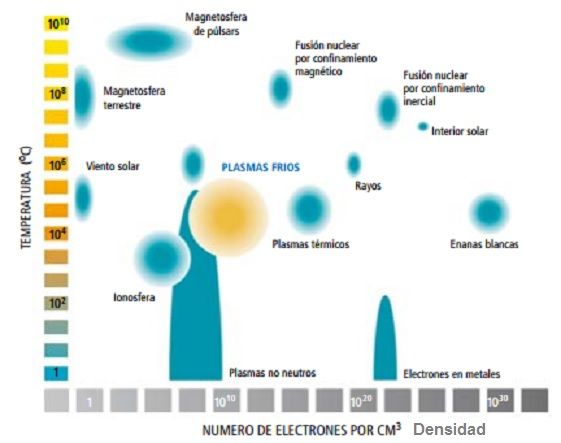
\includegraphics[height=7.8cm]{assets/figures/plasma.jpg}  
    \end{figure*}
